\documentclass[a4paper, 10pt]{ctexart} %中文支持
\usepackage{float}              %防止浮动元素浮动
\usepackage{rotating}           %旋转图片
\usepackage{amsfonts}           %对某一些字体之支持
\usepackage{mathrsfs}           %mathscr e.g.
\usepackage{amsmath}          %数学公式
\usepackage{amsthm}             %定义, 定理, 证明, 例子环境的支持
%使用方法:
%\newtheorem{environment name}{caption}
%比如 \newtheorem{example}{这是例子}
%效果 \begin{example} xxx \end{example} -> 这是例子 1 xxx
%proof就不需要了
\usepackage{graphicx}           %插入图片
\usepackage[left=1.25in,right=1.25in,top=1in,bottom=1in]{geometry}   %用来排版的
\usepackage[]{color}            %给部分文本上色的
%\usepackage{algorithm}          %写伪代码的
%\usepackage{algorithmic}       %同上
%\usepackage{algorithm}
%\usepackage{algorithmicx}
%\usepackage{algpseudocode}
%\usepackage{minted}
\usepackage{amssymb}            %用来加入一些数学符号, 比如说 $\varnothing$
\usepackage{titlesec}
\usepackage{fontspec}           %不知道用来干嘛的
\usepackage{hyperref}           %生成可跳转的书签
% -------------------------------
%\setmonofont{Ubuntu Mono}       %?
%\usemintedstyle{custommanni}    %设置minted插入代码的风格
\titleformat*{\section}{\huge\bfseries}             %管理title的字体和大小
\titleformat*{\subsection}{\Large\bfseries}         %bfseries就是默认的字体.
\titleformat*{\subsubsection}{\large\bfseries}
% -------------------------------
\newtheorem{theorem}{Theorem}
\newtheorem{example}{Example}
\newtheorem{definition}{Definition}
\newtheorem{lemma}{Lemma}
\newtheorem{remark}{Remark}
\newtheorem{corollary}{Comment}
\newtheorem{proposition}{Proposition}
\pagestyle{plain}
\title{Divide\ and \ Conquer\ 第二次课\thanks{可能是第二次课}}
\author{You \and me}

\begin{document}
\maketitle
\tableofcontents
今天我们面对的是Divide and Conquer的算法思想, 基本就是递归调用嘛.
一般都会有递归方程: $T\left(n\right) = a T\left(n / b\right) + f\left(n\right)$
这样的东西. 

前面我们已经学习了很多分析上面递归方程的复杂度的方法, 以及学习了两个经典案例: 归并排序以及快速排序. 今天讲的依旧是这些东西.


\section{what is divide and conquer?}
divide and conquer is a method to solve a question, to design an algorithm.
It has two parts as whose name have suggested: Divide and Conquer. The basic idea is to divide the problem into some subproblems and try to conquer those 
subproblems. 

The precedure consists of three parts in fact. Let's make a list.

\begin{enumerate}
    \item Divide: to divide the problem.
    \item Conquer: try to solve the subproblems
    \item Combine: given the solution of some subproblems, to derive the 
    the solution to the original one from those solutions.
\end{enumerate}

So the outline of the analysis of a divide-and-conquer algorithm is that to find the recurrence function of 
the algorithm, and by using some previous knowledge of recurrence function, to figure the time complexity of the 
algorithm, that is to know: given the scale of input, let's say $n$, the order of $T(n)$ , which stands for 
the time complexity.

It is clear that the operations of division and combination take time. Say that they take $D\left(n\right)$ and $C \left(n\right)$ 
separately. And we assume that the operation of division divides a $n$ scale problem into $a$ subproblems with $n  / b$. Then we can write out 
the recurrence function:
\begin{align*}
    T\left(n\right) = 
    \begin{cases}
        \Theta \left(1\right)  & \text{if} n \le c\\
        a T\left( n  / b \right) + D\left(n\right) + C\left(n\right)&  \text{otherwise}
    \end{cases}
\end{align*}

\begin{corollary}
    There is actually a much more complex and annoying situation, that is what if the division divide 
    a problem into one subproblem with scale $n \times \frac{1}{3}$ and a subproblem with scale $n \times \frac{2}{3}$. So you can not 
    use master theorem.

    How are you going to work this out?
\end{corollary}

\section{排序法}
A sort is an operation to or, let's say, a process of some `unordered sequence', to make it `ordered'. 
\begin{example}
    Give a sequence `$52 , 49 , 80 ,  36  , 14 , 58 ,  61 , 23 , 97 , 75$', after the ordering,
    the output is 
    \begin{align*}
        14, 23 , 36  , 49 , 52 ,  58 
    \end{align*}
    and so on and so on.
\end{example}

\paragraph{the defintion of ordering} We can describe the above intuitive expression with more acuracy.
Let's put it straight. We are given a sequence $\left\{R_{1}, \cdots   ,R_{n}\right\}$. (You know how to precisely define 
a sequence. Check some mathematical analysis textbooks.)

And the sequence has a corresponding sequence of key
\begin{align*}
    \left\{K_{1} , \cdots  , K_{n}\right\}
\end{align*}
which act as an identificator, to determine the position of the order of some $R_{i}$, that is there exists a relation on those keys. (and the relation is partial order relation, and moreover is 
linearly ordered.):
\begin{align*}
    K_{p_{1}} \le K_{p_{2}} \le \cdots  \le K_{p_{n}}
\end{align*}

So what sort do is to reordering the sequence $\left\{R_{1} \cdots \right\}$ into $\left\{ R_{p_{1}}, \cdots \right\}$

\paragraph{The interior ordering and external ordering} When scale of the sequence is so big that the memory can not 
hold it viz. the ordering can not complete within the memory. 
The sort algorithms that work within the memory are called interior sort.

\subsection{the classification of ordering algorithms}
We call the collection of $R$ which are in order as `ordered area', and respectively call the rest the `unordered area'. 

\begin{definition}[round] 
    a round within the algorithm is the operation that enlarge the number of $R_{i}$ that is in order.
\end{definition}

There are 4 basic catergory of ordering algorithm. Let's make a list: 
\begin{enumerate}
    \item insert: to insert some member of unordered area to ordered area
    \item select: to select the highest or lowest in unordered area, and put it right next to order area.
    \item swap: to swap the target in unordered area, and swap it with some other $R$ in unordered area, making it ordered.
    \item merge: given two or more ordered sequence, to merge them into a bigger ordered sequence.
\end{enumerate}
\begin{corollary}
\textcolor{red}{note that the definitions of {\bfseries select} and {\bfseries swap} are wrong}
\end{corollary}

Base on the idea of divide and conquer, we have some prototype of the ordering algorithm. 

One is to select a position basing on which we divide the problem (the description here might be not very clear). 
Another is to choose a member of the sequence, base on which we make a partition where
members that are bigger than it are placed behind while the members that are smaller than it 
are placed in the front.

And the combination operations are indeed different accordingly. 

\subsection{merge sort}
As we have stated, we choose a position can divide the sequence accordingly, by which we get two 
subproblems. 
\begin{definition}
    given the sequence, let describe in the form of array
    $A[i,\cdots, j]$. We divide it with the position $k$. 

    Then we have $A[ i, \cdots    , k  ] A \left[  k + 1 ,  \cdots  , j\right]$ ,where $k  = \displaystyle  \frac{ i  +j}{ 2}$. Then we solve  the subproblems
    recurrently and combine them afterwards. That is merge sort.
\end{definition}
\noindent The key is that we assume the 
$A\left[ i , \cdots ,k \right] , A[k+1 , \cdots  ,j]$ are ordered. And we combine them to make to 
a larger sequence that is ordered.
\subsubsection{code}
Figure~\ref{fig:merge1} shows the pseudo-code of merge sort. The main idea 
is merge, which use the idea of pointers.
\begin{figure}[]
    \centering
    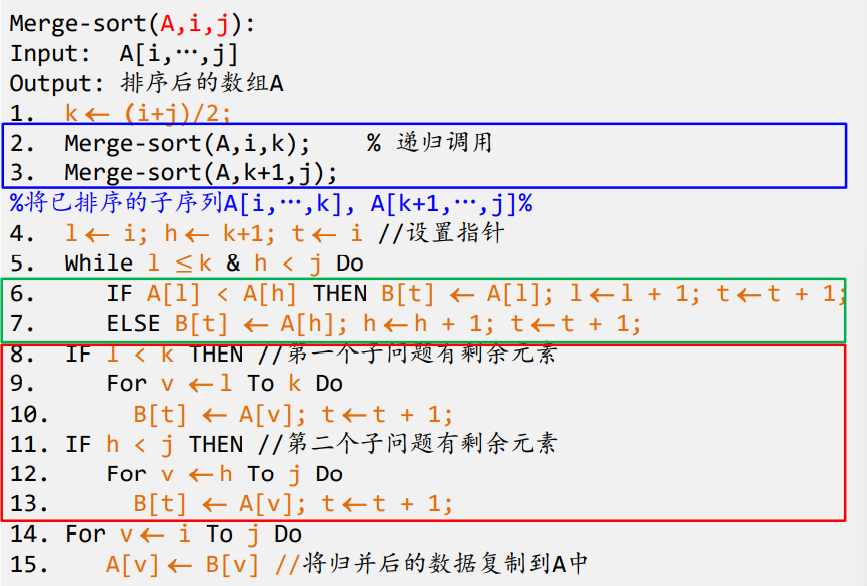
\includegraphics[scale = 0.5]{merge1.png}
    \caption{code of merge sort}
    \label{fig:merge1}
\end{figure}
\subsubsection{analysis}
We can easily write out the recurrence function of the 
algorithm: 
\begin{align*}
    T \left( n\right)  = 
    \begin{cases}
        2  T(  n / 2) + n & \\
        O\left(1\right) & n< c
    \end{cases}
\end{align*}
Because, operation that combine the two sequences need 
$\Theta \left( n\right)$ costs. And then we use master theorem:
\begin{align*}
T \left( n\right)  =  \Theta \left( n \log n\right)
\end{align*}
\subsection{快速排序}
the sketch of the algorithm is that 
we choose a $x$ and parition the sequence 
basing on it. 
Then we have two subproblems and deal with them 
in the same way. Then we will have the answer.
\subsubsection{the code}
\begin{figure}[htbp]
    \centering
    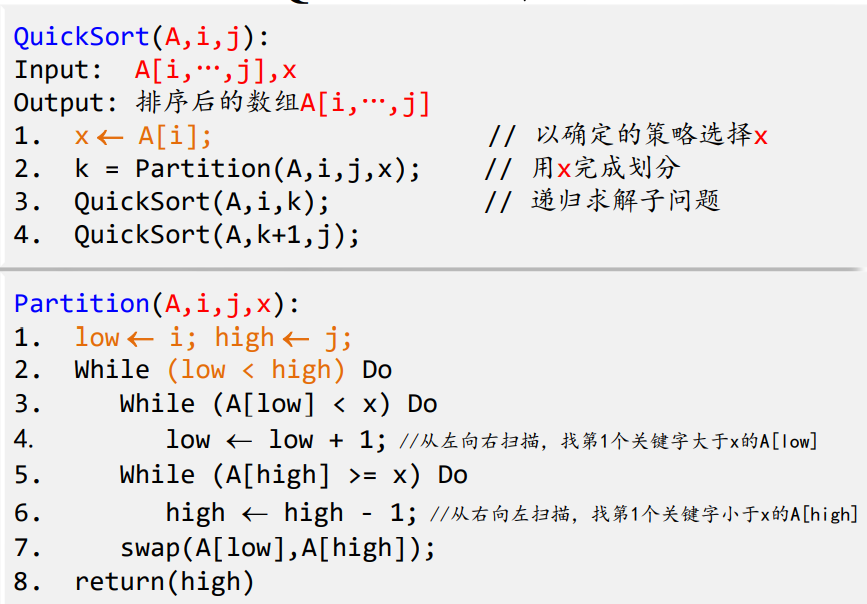
\includegraphics[scale = 0.5]{quicksort1.png}
    \caption{the pseudo code of quick sort}
    \label{fig:quicksort1}
\end{figure}
Figure~\ref{fig:quicksort1} shows the pseudo code of the quick sort.
\subsubsection{the time complexity analysis}
\paragraph{worst case}The time it takes in the worst case is :
\begin{align*}
    \Theta \left(n ^{2}\right)
\end{align*}
let's say we are given an ordered sequence but in a reverse order. So every partition takes a 
long time, like $\Theta \left(n\right)$ where it have to compare to every other member of the 
sequence. More precisely, for the first chosen $x$, the partition takes $n-1$ operations. For the $i$ th $x$, the partition 
takes $n - i$ operations. 

The time algorithm cost is consequently $\Theta \left(n^{2}\right)$

\paragraph{best case} % (fold)
\label{par:best case}
every time the scale of the subproblems are equal in a best case, which result to that 
the recurrence function is that 
\begin{align*}
    T\left(n \right) =  2 T(n  /2    ) + \Theta \left(n\right)
\end{align*}
We can use master theorem to figure that  $T\left(n\right) = \Theta \left(n \log n\right)$
% paragraph best case (end)

\paragraph{average case} % (fold)
\label{par:average case}
the average case is actually $\Theta \left( n \log n    \right)$ the same to the best case. It is not saying that they have the same costs.

If we consider the scale of subproblems, the `average' can be viewed as follows:
\begin{align*}
    \frac{1}{n} \sum_{s=1} ^{n} \left(T\left(s\right) + T \left(n  -s\right)\right) 
\end{align*}
Because the case where scales differ have actually equal chances to happen. 

Consequently, we have 
\begin{align*}
    T\left(n\right) & = \frac{1}{n} \sum_{ s = 1}  ^{n} \Big(T\left(s\right) + T\left( n -s\right)\Big) + cn\\
    & = \frac{1}{n} \left( 2 T \left(1\right) + \cdots  + 2 T\left( n -1\right) + T \left(n\right) \right) + cn
\end{align*}
Here is some technique we need to use : 
\begin{align*}
    \left(n  - 1\right) T\left(n\right) =  2 T\left(1 \right)  + 2 T\left(2\right)  +\cdots  + 2 T\left(n-1\right) + c n^{2} \tag{1} \\
    \left(n-2\right)  T\left(n - 1\right) =  2 T\left(1\right) + \cdots  + 2 T\left( n  -2   \right) + c \left(n - 1\right) ^{2} \tag{2} 
\end{align*}
substract equation (2) from equation (1) . Anyway, we have 
\begin{align*}
    \left(n  - 1\right) T\left(n\right)  -  \left(n  -2\right)  T\left( n -1\right)  = 2 T\left(n - 1\right) +c \left(2 n - 1\right)  \\
\end{align*}
which leads to 
\begin{align*}
    & \left(n - 1\right) T\left(n\right)   - n T\left( n -1\right) = c \left( 2n -1 \right) \\
    \implies & \frac{T\left(n\right) }{ n}  = T\left( n-1   \right) / \left(  n -1\right) + c \left( \frac{1}{n} + \frac{1}{n-1}\right)
\end{align*}
which allows us to calculate the value of $T\left(n\right) $ recurrently, viz. 
\begin{align*}
    T \left(n\right) / n & = c \left( \frac{1}{n} + \frac{1}{n -1} \right) + c \left( \frac{1}{n-1} + \frac{1}{n-2} \right) + \cdots  + c \left(\frac{1}{2} + 1 \right) + T (1 ) \\
    & = c \left( \frac{1}{n } + \frac{1}{n-1    } + \cdots + \frac{1}{2} \right) + c \left( \frac{1}{n-1} + \frac{1}{n-2} + \cdots   + 1\right)  + T\left(1\right)
\end{align*}
These two parts are same. There is no need to separate them like what we have done here.

Next, we use a asymptotical analysis of Harmony series, viz.
\begin{align*}
    H_{n} & = 1 + \frac{1}{2} + \cdots + \frac{1}{n} \\
    & = \log n + \gamma + \frac{1}{2n}  -\frac{1}{12n ^{2} } + \frac{1}{120 n^{4} } - \varepsilon
\end{align*}
where $ 0 < \varepsilon < \frac{1}{252n ^{6} } $ , and gamma is euler const. Just forget about that. This proposition is too strong. Anyway, it is crystal clear that $H_{n} =  O \left(\log n\right)$. So apparently, 
\begin{align*}
    & T\left(n\right) / n  = c \left(H _{n} - 1\right)  + c H_{n-1}  = O\left(\log n\right)
\end{align*}
then we have 
\begin{align*}
T(n) = O\left(n \log n\right)
\end{align*}

% paragraph average case (end)
\subsubsection{random quick sort}
In the algorithm above, we can notice that the worst case happens when the sequence 
is in reverse order. That is because the chosen $x$ is the first member of the sequence. 
Consequently, a natural way to improve the algorithm, is to randomly choose the $x$, in the
partition operation.

Thus for different sequences, they have the same expectation of the time it consumes.

That was great. 

\paragraph{the code} % (fold)
\label{par:the code}

the code is left to the readers as exercise, because it is 
very easy. Just a slight change.
% paragraph the code (end)

\paragraph{analysis} % (fold)
\label{par:analysis}

Here is some notation: 
\begin{definition}
    $S_{\left(i\right)}$ stands for the $i^{\text{th}}$ smallest element. For example $S_{\left(1\right)}, S_{\left(n\right)}$, the former is smallest member, and latter is the biggest member. 

    $X_{ij}$ is a random variable, defined as follows: 
    The value of $X_{ij}$   
    is equal to the number of the comparison between $i , j$ 
    in the algorithm. 

    Consequently, the comparison made during the algorithm is 
    \begin{align*}
        \sum_{i  =1}  ^{n} \sum_{j > i}  X_{ij}
    \end{align*}
    Note that it is still a random variable.
\end{definition}

Consequently, what we want to know is the expectation of the series above,
viz. 
\begin{align*}
    E \left[ \sum_{i=1} ^{n} \sum_{j > i}  X_{ij} \right] = \sum_{i=1}^{n} \sum_{ j > i}  E\left[ X_{ij} \right]
\end{align*}

Actually the 
$X_{ij}$ can only have the value of 
$0 $ and $ 1$, which leads to that 
$E \left[ X_{ij} \right] =  p_{ij} \times 1 + \left(1-  p_{ij} \right) \times 0$.
So the question is to find $p_{ij}$

In a partition, the chosen $x$ has to be compared to every 
other members in the sequence.
Moreover, once the partition is over, 
$x $ will not be compared again. Now you should know why the value of $X_{ij}$ can only be $1 $ or $0$.

Every operation of partition, actually, will form a partition of 
the sequence. May you can draw some pictures to figure this out.
Anyway, two members, let's say $i$ and $j$, can be compared only when they are 
in `a' same class of the parition (the class is short for equivalent class). 

The analysis can be carried on now. Please take a notice to the next procedure of analysis: 
\begin{enumerate}
    \item Only when $S_{i} , S_{i + 1} , \cdots  , S_{j}$ is in a same class, $S_{(i)}$ and $S_{\left(j\right)}$ can be compared.
    \item Only when $S_{\left(i\right)} $ or $S_{\left(j\right)}$ is chosen as the $x$, these two can be compared.
    \item Moreover, if we choose some $S_{\left(k\right)}$ where $k< i$ or $k > j$, $S_{(i)}, S_{(j)}$ are still possible to be compared.
    \item The probability of $S_{\left(i +k\right)}$ to be chosen as $x$ are equals. So the probability of $S_{\left(i\right)} , S_{\left(j\right)}$ to be chosen as $x$ is 
    \begin{align*}
        \frac{2}{ j   - i + 1}
    \end{align*}
    viz. 
    \begin{align*}
        p_{ij} =  \frac{2}{ j  -i + 1}
    \end{align*}
\end{enumerate}
\begin{remark}
    One might notice that the number of members in the class might not be precisely the $j - i + 1$.
    We just ignore this situation. Why?
\end{remark}

It is available to calculate the expection now. 
\begin{align*}
    \sum_{i=1} ^{n} \sum_{ j >  i }  E \left[ X_{ij} \right] & 
    = \sum_{i=1} ^{n}\sum_{j > i}  \frac{2}{j - i  +1} \\
    & \le \sum_{ i = 1}  ^{n} \sum_{k=1} ^{n  - i + 1} \frac{2}{k} \le 2 \sum_{i=1} ^{n} \sum_{ k =1} ^{n - i  + 1} \frac{1}{k} \\
    & = 2n H_{n} = O\left( n \log n\right)
\end{align*}

Over ! 
% paragraph analysis (end)

\subsection{the lower bound of sort problem}
It describe how fast the sort can be under certain cases.
For example, under the worst case or under the average case.

\begin{definition}
    If a problem has a low bound, for example, $\Omega\left( n\log n\right)$, 
    and if the time complexity of an algorithm is 
    $O \left( n\log n\right)$, 
    then we say that 
    algorithm is optimal.
\end{definition}
\begin{definition}[decision trees]
    A procedure and the all the cases of a sort can be expressed as tree,
    where, the leaf nodes stands for the resulted sequences.
    and the non-leaf nodes stands for the operations of comparsion.

    And moreover, the number of the non-leaf node in a path stand of the 
    comparison it shall take under this case. 
    That is the level of the leaf stands for the number of operations.
\end{definition}

Thus, the low bound of a sort, is the lowest level of a leaf. 


let's say that the decision tree has height $h$ and have $l$ leaves. All the possible resulted sequences are in number of 
$ n !$.

Then we can easily get an inequality :
\begin{align*}
      n ! \le l \le 2 ^{h}
\end{align*}
Then
\begin{align*}
h \ge \log \left( n !\right) = \Omega \left( n \log n\right)
\end{align*} 
We can see that
\footnote{the approximation can be deduced from Stirling formula: $n ! \sim \sqrt{2\pi n} \left( \frac{n}{e}\right) ^{n}$}
, in the worst case, the 
time complexity has a low bound $\Omega \left( n \log n \right)$

%====================================
\paragraph{the average case} % (fold)
\label{par:the average case}
we consider the average length of paths, which is that 
\begin{align*}
    \frac{ \text{total length}}{n !}
\end{align*}
when the decision tree is \textbf{balanced}, the average length above takes minimum. 

\begin{definition}[balanced decision tree]
In a balanced decision tree, every leaf has level either $d$ or $d - 1$, where $d$ is the 
height of the tree.
\end{definition}

Because what we want is a lower bound. So 
only the balanced decision tree is concerned,
which is the minimum, which is, what we want. 

\begin{enumerate}
    \item it is clear that $d = \left\lceil \log  c \right\rceil$, where $c = x_{1} + x_{2}$
    \item $x_{1}$ in level $d - 1$ and $x_{2} $ in level $d$
    \item $x_{1} + \dfrac{x_2}{2} = 2^{d-1}$. $2 ^{d- 1}$ is the number of nodes in 
    level $d  -1$
    \item total length:
    \begin{align*}
        M & = x _{1} \left(d - 1\right)  +x_{2} d  \\ 
        & = \left(2 ^{d} - c     \right) \left(d - 1\right) + 2 \left( c - 2 ^{d-1}\right) d \\
        & = c \left(d - 1\right) + 2 \left( c - 2 ^{d-1}\right) \tag{$d- 1  = \left\lfloor  \log c \right\rfloor$} \\
        & = c \left\lfloor \log  c \right\rfloor + 2 \left(c - 2 ^{\left\lfloor \log c \right\rfloor}\right)
    \end{align*}
    \item $c = n!$ since this is the case when the tree has lowest height. 
    \item We claim that $c  - 2 ^{\left\lfloor \log  c \right\rfloor } \ge \dfrac{c}{2}$ so 
    \begin{align*}
        M / n ! & > \left\lfloor \log n ! \right\rfloor + 1 \\
        & = \Omega \left( n \log  n\right)
    \end{align*}
    \item so the low bound in average case is $\Omega \left( n \log n\right)$
\end{enumerate}
% paragraph the average case (end)

In general, the low bound of sort is $\Omega \left( n\log n\right)$ in all possible cases.
The quick sort is optimal when the const is ignored.

Oh my god! I mean, this is bad. The deduction is like shit.
\section{MAX and MIN 问题}
\noindent\textbf{Input}: $n$ 个互异的数组成的数组 $A$ , 以及一个正整数 $i$

\noindent\textbf{Output}: $B = \left\{ x | \left| A \le x \right| = i \right\}$
for this proposed problem, if it is sovled, then the Max  と Min can be solved.

我们想到的最简单的方法很明显就是直接排序然后进行一个选取, 但是这样未免有点简陋了, 并且效率也是一点也不理想. So we may tackle the 
simplified problem here: find the Max と Min.

\subsection{算法1, 不使用递归方程}
一个明显的想法就是直接从头到尾扫描两边, 就都求出来了, 时间复杂度是 $2 \left(n-1\right)$ , 其中 $n$ 是问题的规模, 在这里是数组的大小.
我们这里能够给出一个算法, 其效率是 $\displaystyle \left\lfloor \frac{n}{2} \right\rfloor   +  2 \left\lceil \frac{n}{2} \right\rceil$: 

\begin{enumerate}
    \item 从数组的两端开始, 两两比较, 将较大的一方放在前面, 较小的一方放在后面
    \item 我们能够知道, 最大值一定在前面, 最小值一定在后面
    \item 我们分别扫描前面和后面, 就能够得出最大值和最小值了
\end{enumerate}
我们对这个算法进行一下分析

1. 中执行次数其实只有 $\lfloor \dfrac{n}{2} \rfloor$ , 
这是因为当 $n$ 是奇数的时候, 中间的数字不需要变动, 因为算要变动也是自己和自己交换
, 于是向下取整;

3. 中分别扫描 $A \left[ 1, \cdots  ,  \lceil \dfrac{n}{2} \rceil \right]$,
以及 $A \left[ \lceil \dfrac{n}{2} \rceil , \cdots   , n \right]$, 
就能分别求出最大值和最小值了, 
比较的次数是 $2 \lceil \dfrac{n}{2} \rceil$. 于是时间复杂度就是 
\begin{align*}
\displaystyle \left\lfloor \frac{n}{2} \right\rfloor   +  2 \left\lceil \frac{n}{2} \right\rceil
\end{align*}

\newpage
这个证明并不是很会捏, 这里给出伪代碼:
\begin{figure}[H]
    \centering
    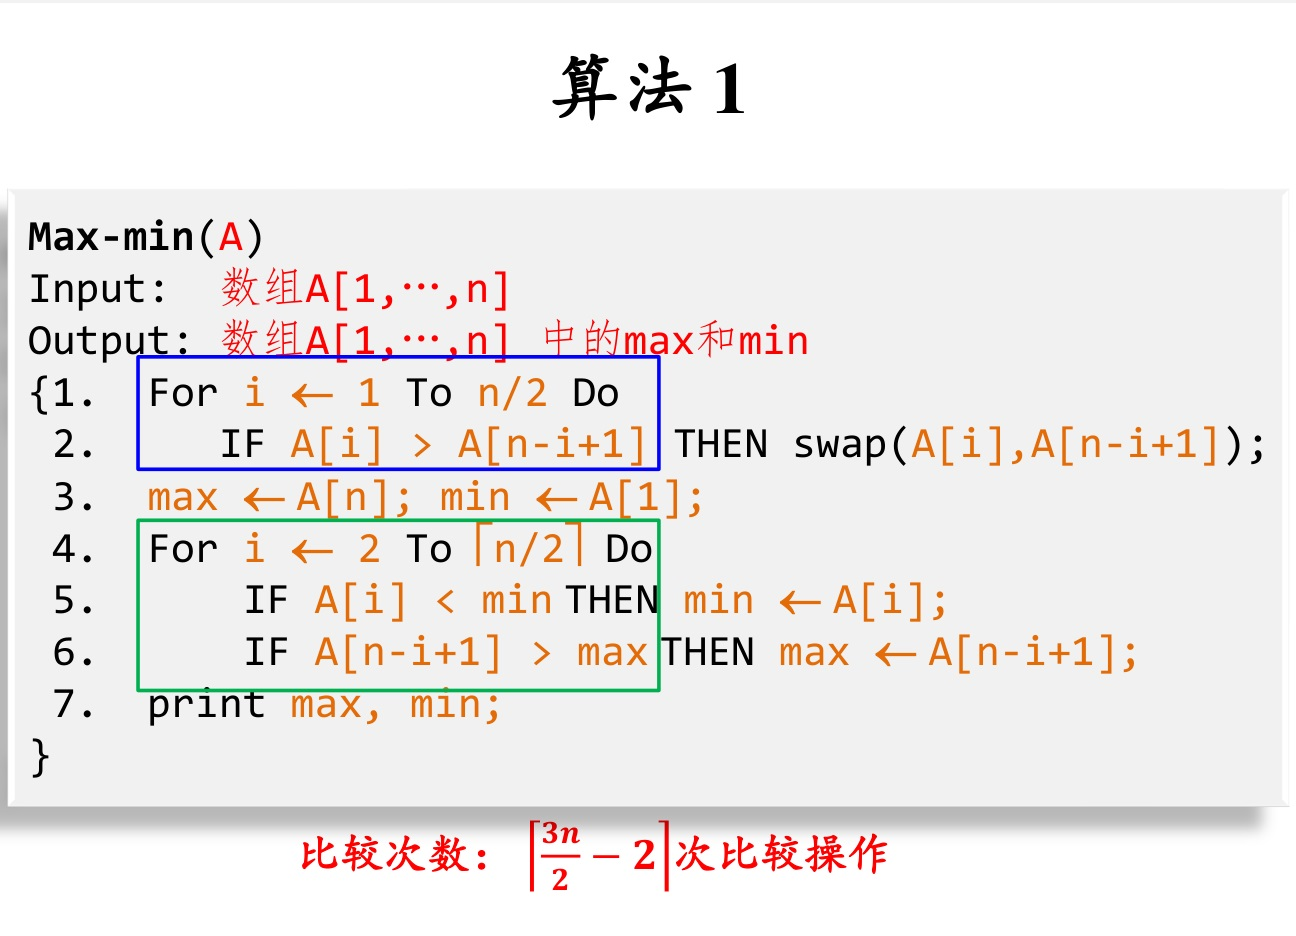
\includegraphics[scale=0.3]{1.jpg}\caption{不使用遞歸方程的算法}
\end{figure}
\subsection{算法2, 使用递归方程}
\begin{enumerate}
    \item line 1 と 2 are initial value of recurrence function. 
    \item line 6 \& 7 are division. 
    \item line 8 \& 9 are combination.
\end{enumerate}
\begin{figure}[H]
    \centering
    \includegraphics*[scale = 0.3]{2.png}\caption{使用遞歸方程的算法}
\end{figure}

图中的算法是一个递归求解的过程, 将规模为 $n$ 的问题转化为两个 $n / 2$ 的问题, 
即求出前半的最值, 后半的最值, 而后进行比较, 得出总的最值
, 能够得出:
\[
T\left(n\right) = 2 T\left(n /2\right) + 2
\]

下面我们来看看这个的时间复杂度, 设 $n = 2 ^{k}$
(因为这样方便一点) , 
\[
\begin{aligned}
    T\left(n \right)& = 2  T\left(n /2\right) +2 \\
    & = 4 T\left(n / 4\right) + 2 ^{2} +2 \\
    & = 2 ^{3}T\left(n / 8\right) + 2 ^{3} + 2 ^{2} +2 \\
    & = \cdots \\
    & = 2^{k-1} T\left(2\right) + \sum_{i=1} ^{k-1} 2 ^{i}
\end{aligned}
\]
\noindent \textbf{Remarks.} \\
1. $T\left(n\right) = 2 T\left( n /2\right) + 2$ 
后面常数是   $2$ , 是因为最大值和最小值各比较一次\\ 
2. 如何计算的? $2 T\left(n /2 \right) = 
2\left(2 T\left( n /4\right) + 2\right) + 2 
= 4 T\left( n / 4\right) + 2 ^{2 +2} \cdots$\\
3. 不再研究最大最小值选择问题的下界和平均情况下选择的下界 
(为什么?\footnote{这并不是留给读者思考的, 我是真不知道为什么})

\section{选择中位数} 
\subsection{问题描述}

\noindent \textbf{Input} : 一个长度为 $n$ 的数组\\
\textbf{Output} : 这个数组的中位数\footnote{
    选取第 $\left\lfloor \dfrac{n+1}{2} \right\rfloor$ 大的数字}
\subsection{算法设计}
直接给出算法:{\sffamily Select (A, i)}的定义

参数 $A , i$, 其中 $A$ 是数组, $i$ 
定义为 $\left\lfloor \left(n +1\right) / 2 \right\rfloor$, 意为选择数组中第 $i$ 大的数字
\\
\noindent step1. 将我们的数组分为五个部分
\\step2. 使用插入排序将这个五个部分排序, 以此选出五个中位数
\\step3. 在这五个数字中递归调用算法 {\sffamily Select}\footnote{Select 之中使用 Par}, 得出中位数, 记为 $x$ 
\\step4. 使用函数划分 {\sffamily Partition}: 将所有小于 $x$ 的放在前面, 
大于 $x$ 的放在后面. 并且得到 $x$ 的下标 $k$
\\step5. 将下标 $k$ 和 $i =  \left\lfloor \dfrac{n+1}{2} \right\rfloor$ 比较
\\如果说 $i = k$ 则 OK , 如果说 $k > i$ , 则在前面寻找第 $i$ 大的数, \\
\begin{figure}[H]
    \centering
    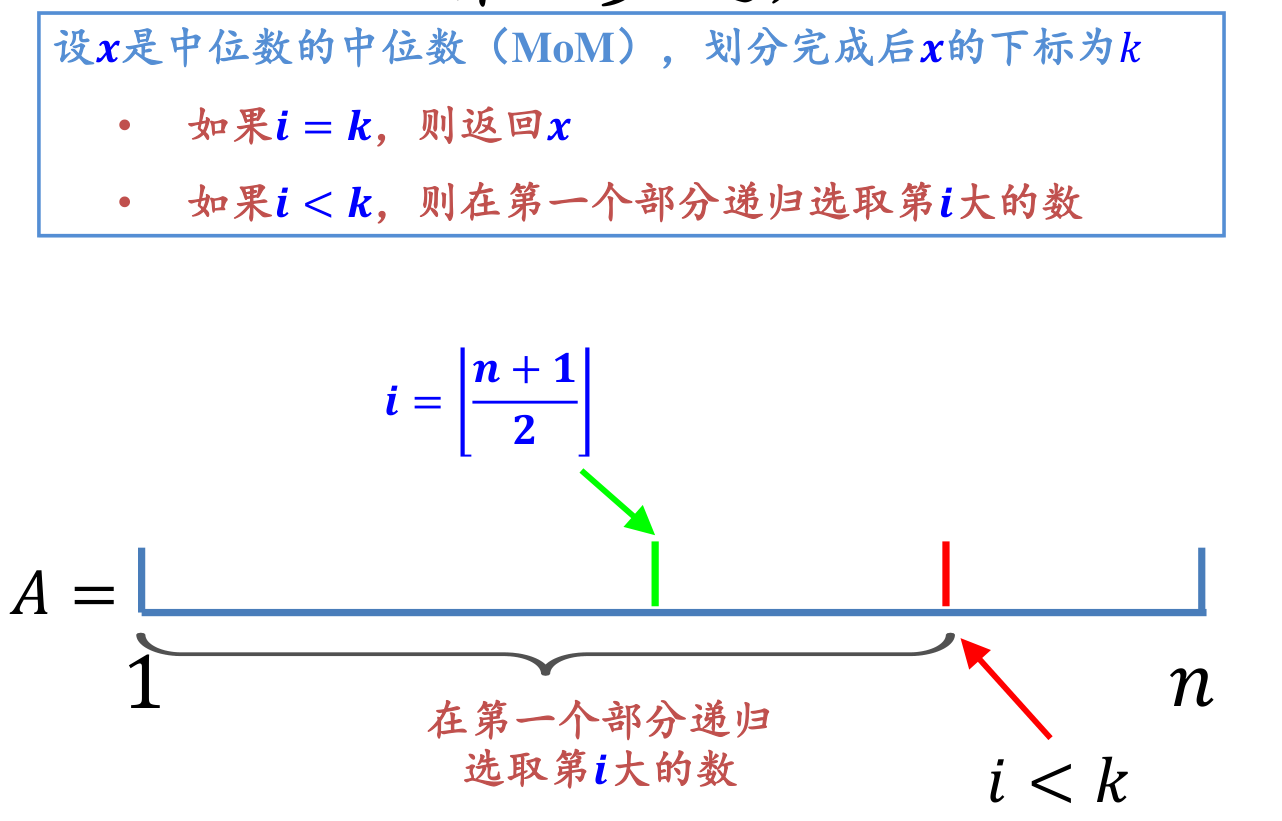
\includegraphics[scale = 0.3]{4.png}\caption{}
\end{figure}
如果说 $k < i$ 则在后面寻找一个 $i - k$ 大的数.\\
\begin{figure}[H]
    \centering
    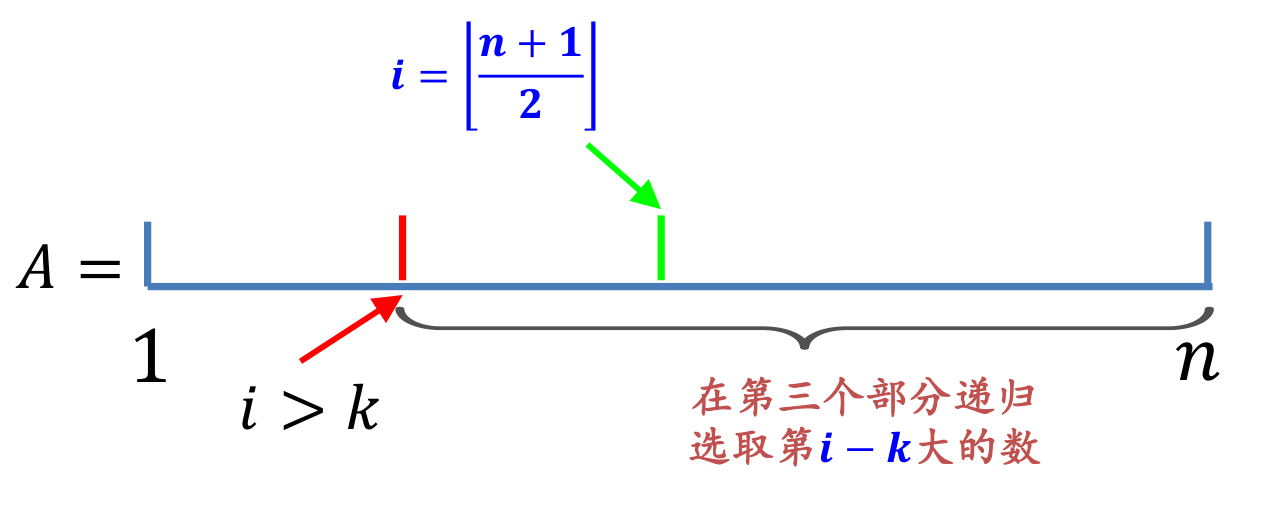
\includegraphics[scale = 0.3]{5.png}\caption{}
\end{figure}

\subsection{伪代碼}
\begin{figure}[H]
    \centering
    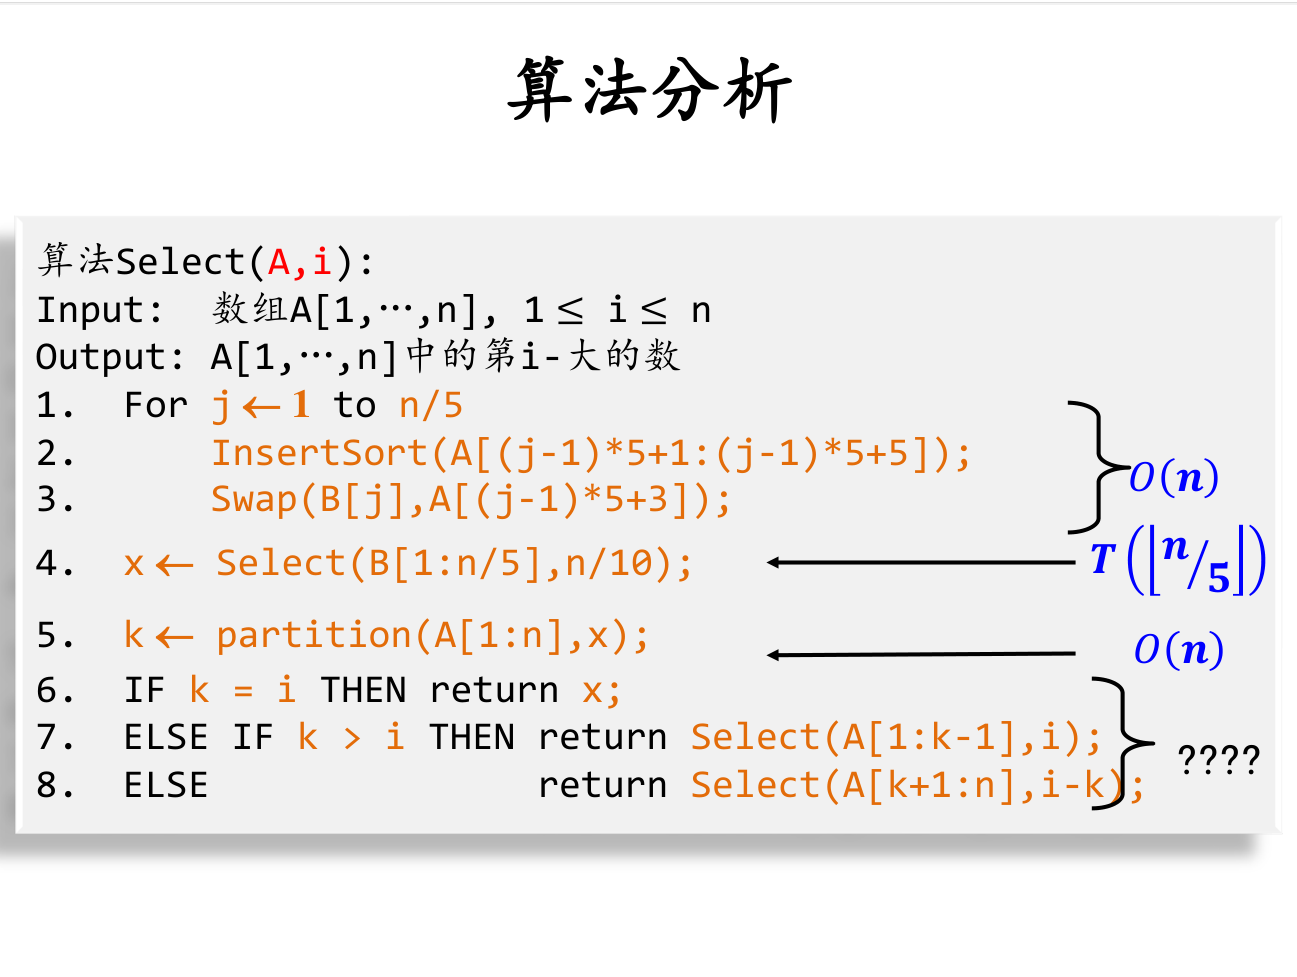
\includegraphics[scale = 0.3]{3.png}\footnote{这里需要一些修改}\caption{}
\end{figure}
这个东西是不是没有设置初始条件阿? 比如说我有一个长度为 5 的数组, 然后输进去之后还要调用这个 
select 吗? 搞不懂啊.

总之, 这个算法的流程就是, 我重复一下上面的这个东西. 这个算法实际上是将, 这个数组, 预处理一下, 选择出一个怀疑对象, 
这个预处理使用的是这个 insertion sort; 而后是 divide \& Conquer 的部分, 重复使用 partition 得出答案. 

但是这里有一个问题, 我们的算法是不是没有处理初始情况? 
\subsection{select 的一个估计}
就是说, 我们将这个members, 什么 members 呢? 就是那些, 可能被上面 line 6 7 之类删掉的那些数字. 排成一个矩阵, 如果说 $a _{ij}$ 来表示矩阵元素. 并且, 总共有 5 列. 
每一列都有 $ n / 5$ 个元素. 大概是这个数字, 当这个 $n$ 很大的时候, 就能够忽略这个余数带来的差别. 

总之这个时候我们要看那个ppt, 那个ppt 上的红色标识的元素, 实际上就是, 得出的那个下标的元素, 面对这些东西, 我们能够看出. 
这里面的, 虚线框的东西, 就是我们可能剔除掉的东西, 我们对这个数字进行一个估计, 我们估计, 删掉的元素实际上最少有 

\begin{align*}
    \left\lfloor \frac{3n}{10} \right\rfloor
\end{align*}

这是因为, 这个时候, 对于一个矩阵成员, $a_{\mu \nu}$ , 如果说 $ \mu \le i , \nu \le j$ 我们断言, 这个 $a_{\mu\nu} \le a_{ij}$.
这里我们进行了一个非常粗糙的估计: 这里, 减少的成员, 大概有
\begin{align*}
    \left\lfloor \frac{3n}{10} \right\rfloor
\end{align*}

这是一个比较缺少考虑的估计, 我们能够明显地举出反例. 但总之, 这些技术细节, 并不是很重要. 我们知道一个大概就行: 
\begin{align*}
    n  - \left\lfloor \frac{3n}{10}\right\rfloor \le \frac{7n}{10}   +6 
\end{align*}

因此递归调用的操作的复杂度至多是 $ T \left( \frac{7n}{ 10} + 6\right)$. 于是我们能够就此得到递归方程: 
\begin{align*}
    T \left(n \right) =  
    \begin{cases}
        \Theta \left(1\right) & n \le c \\ \\
        T \displaystyle \left( \left\lfloor  \frac{n}{5} \right\rfloor \right) + T \left( \frac{7n}{10} + 6\right) + \Theta \left(n\right) & \text{otherwise}
    \end{cases}
\end{align*}
于是说, 时间复杂度就是 
\begin{align*}
    T \left( n \right) =  O \left( n \right)
\end{align*}
线性时间内就能够完成. 非常好算法.

\section{大数乘法}
废话不多说 

我们要做的就是两个大数相乘, 使用类似的方法 (二分) , 转化为几个子问题

为了提高效率, 这两个大数是以二进制表达的\footnote{下面用到的左移操作, 在计算机中只需要常数时间}
\\ [8pt]
\subsection{问题描述}
\noindent\textbf{Input} : n 位二进制整数 $X , Y$ \\
\textbf{Output} : $X, Y$ 的乘积 \\
我们正常一位一位计算需要的时间复杂度是 $O\left( n^{2}\right)$\footnote{为什么是
$O$ 符號呢, 你看如果说这个大数里有很多 $0$, 就不需要算那么多次了} (一位数乘以 $n$
位整数是 $O \left(n\right)$ 的时间, $n$ 位数乘以 $n$ 位数就是 $O (n \times n  
)$的时间), 但是我们用 Divide and Conquer 
可以得到复杂度为 $O\left( n ^{\log_{2} 3}\right)\approx O\left( n ^{1.59}\right)$ 的算法.
\subsection{简单的 Divide and Conquer 算法}
将 $X$ 记为 $A\ |\ B$, 其中 $A, B$ 是两个 $n / 2$ 位的数字, 
$X$ 实际上等于 $A$ 左移 加上 $B$:
\[
X = A \times 2 ^{n /2} + B 
\]
类似地, $Y$ 记为 $C\ | \ D$. 于是就有:
\[
\begin{aligned}
XY &= \left(A \times 2^{n /2} + B\right) \times 
\left( C \times 2^{n /2} +D  \right)\\
& = AC \times 2 ^{n} + \left(AD + BC\right) \times 2^{n /2} + BD
\end{aligned}
\]
根据这个等式我们有第一个算法:\\
1. 计算 $A,B,C,D$\\
2. 计算 $AC, BD$\\
3. 计算 $AD + BC$\\
4. $AC$ 左移, $\left(AD + BC\right)$ 左移 $n / 2$ 位\\
5. 计算 $XY$\\
显然, 1. 只需要常数时间; 2. 递归调用函数 需要 $2T(n /2)$ 的时间; 3. 也是递归调用, 
同时加法需要 $\Theta \left(n\right)$ 的时间;
4. 左移, 常数时间;
5. 计算 $XY$ 使用加法, $\Theta \left(n\right)$ 时间

故
\[
T\left(n\right) = 4 T\left( n / 2\right) + \Theta \left(n\right)
\]
运用Master定理: $T\left( n\right) = \Theta \left(n ^{2}\right)$

\subsection{改进的Divide and Conquer 算法}
我们可以将这个等式简化一下:
\[
\begin{aligned}
XY &= \left(A \times 2^{n /2} + B\right) \times 
\left( C \times 2^{n /2} +D  \right)\\
& = AC \times 2 ^{n} + {\color{red}\left(AD + BC\right)}\times 2^{n /2} + BD\\
& = AC \times 2 ^{n} + {\color{red} \big(\left(A- B\right) \left(D -C\right)
+AC +BD\big)}  \times 2 ^{ n  /2} +BD
\end{aligned}
\]
利用上了已经计算了的 $AC, BD$ 来计算中间这块, 明显
\[
T\left(n\right) = 3 T\left( n / 2\right) + \Theta \left(n\right)
\]
特别地, 当 $n=1$ 时, $ T\left(n\right) = \Theta \left(1\right)$. 
一算就有: $T\left(n\right)= n ^{\log _{2} 3 } \approx n ^{ 1.59}$

\subsection{思考} 能否利用这个想法实现矩阵乘法问题?

感觉可以, 但是我不会.
\newpage
\section{简单的ChessBoard问题}
\subsection{问题描述}
在一个 $2 ^{k} \times 2 ^{k}$ 个方格组成的棋盘中,有一个方格与其它的方格不同,称之为奇异块。\\
要求:若使用以下四种L型骨牌覆盖除这个奇异块的其它方格,覆盖过程中L型骨牌间不能有互相覆盖,
设计算法求出覆盖方案。四个L型骨牌如下图\footnote{你可以看出这个问题一点也不一般化}\\
\begin{figure}[H]
    \centering
    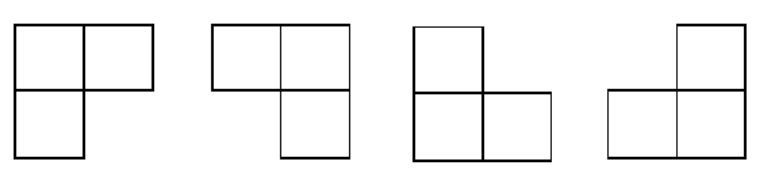
\includegraphics[scale = 0.3]{6.png}\caption{}
\end{figure}
\subsection{算法设计} 
1. 当𝑘 > 0时,将 $2 ^{k} \times 2^{k} $ 的棋盘分成四块 $2^{ k-1} \times 2^{k-1}$ 的子棋盘

2. 使用一个合适的L型骨牌,覆盖三个没有特殊方格的子棋盘的相邻方格

3. 继续递归处理4子棋盘,直到子棋盘中只有一个特殊方格为止

我们将自己得到的算法记为 {\sffamily ChessBoard(tr, tc,dr,dc, k)}\\
其中 {\sffamily tr, tc} 棋盘起点 (最左上) 的坐标 , {\sffamily dr,dc} 是特殊点的坐标,
{\sffamily k} 是棋盘之大小. \\
总体思路是这样\\
1. 划分棋盘为四个象限\\
2. 确定特殊点在那个象限\\
3. 将牌放在中心, 使得牌和特殊点所在的象限无交点\\
\begin{figure}[H]
    \centering
    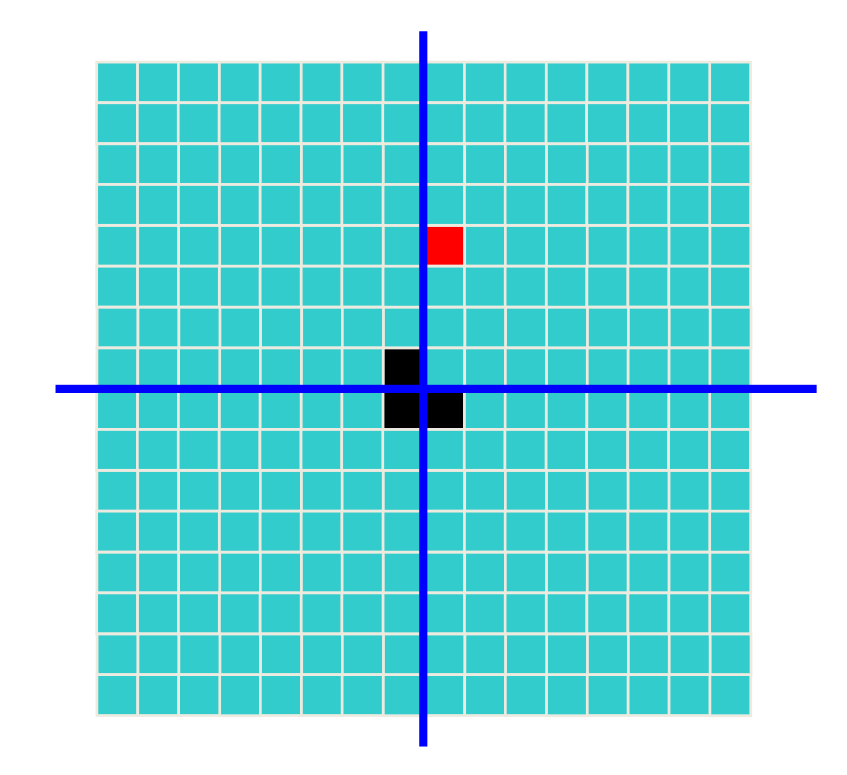
\includegraphics[scale = 0.3]{7.png}\caption{}
\end{figure}
\noindent 4. 将骨牌的各个点视为特殊点\\
5. 得到了四个子问题, 将参数传进递归调用的函数里\\
\begin{figure}[H]
    \centering
    \includegraphics*[scale = 0.3]{8.png}\caption{}
\end{figure}
6. OK
\subsection{算法设计的伪算法}
\begin{figure}[H]
    \centering
    \includegraphics*[scale = 0.5]{9.png}\footnote{ {\sffamily tile =1//被覆盖的方格的记号 }{\sffamily board[$2^k$][$2^k$]储存记号用的数组}}\caption{}
\end{figure}
\subsection{复杂度分析}
我们根据上面的伪代码找出 recurrence function: 
\begin{align*}
    T \left(k\right) = 
    \begin{cases}
        \Theta \left(1\right)    & k =  0 \\ 
        4 T \left( k- 1\right)  + \Theta \left(1\right) & k > 0\\
    \end{cases}
\end{align*}

then we use some simple techniques to work this out 
\begin{align*}
    T \left(k\right) & =  4 T\left( k -1\right)  + \Theta (1) \\ 
    & = 4 \left( 4 T\left( k -2\right) + \Theta \left(1\right) \right) + \Theta \left(1\right) \\
    & \vdots\\
    & =  4 ^{k } T \left(0\right) + \Theta \left(1\right) \sum_{  i= 0}  ^{k - 1} 4 ^{i}\\
    & = \Theta \left(4 ^{k}\right) 
\end{align*}
\end{document}